\chapter{Projekt aplikacji}\label{ch:project}

W tym rozdziale przedstawię wszystkie wymagania funkcjonalne, które powinna spełniać aplikacja, aby użytkownik miał możliwość stworzyć graf dowolnego typu, wyświetlić go w optymalny sposób (wraz z możliwością zmiany widoku) oraz zmienić graf w dowolny sposób, np. poprzez dodawanie nowych wierzchołków i krawędzi, czy edycję etykiet. 

Opiszę również wymagania niefunkcjonalne, aby praca z grafami była możliwie przystępna. Uwzględnię m.in.: wydajność, wspierane platformy, wygodną obsługę przez użytkownika oraz łatwą rozszerzalność dla programistów (co zostanie osiągnięte na przykład poprzez modułowowść kodu w JavaScript).

Na koniec rozdziału zaprezentuję prototyp graficznego interfejsu użytkownika uwzględniającego wszystkie wymagania funkcjonalne, który będzie obrazował jak powinna wyglądać aplikacja tworzona w ramach tej pracy. 

\section{Wymagania funkcjonalne}

\subsection{Tworzenie grafów}
Podstawowym i oczywistym wymaganiem jest, aby użytkownik mógł stworzyć nowy, pusty graf skierowany oraz nieskierowany. Ponadto użytkownik powinien mieć możliwość zaimportowania istniejącego grafu oraz wygenerowania znanego grafu, np. cyklu lub grafu pełnego o zadanej ilości wierzchołków. 

\subsubsection{Importowanie grafów} \label{subsubsec:import}
Użytkownik powinien móc wczytać graf z komputera lub z chmury (np. Google Drive lub Dropbox) w trzech znanych formatach: 

\begin{itemize}
\setlength\itemsep{0em}
\item \texttt{GraphML},
\item \texttt{GEXF},
\item \texttt{JGF}.
\end{itemize}

Opisy formatów znajdują się w sekcji \ref{sec:graph-formats}.

\subsubsection{Generowanie grafów}

Użytkownik powinien mieć możliwość wygenerowania znanych grafów, dla zadanych parametrów wejściowych:

\begin{itemize}
\setlength\itemsep{0em}
\item grafu pustego,
\item grafu liniowego,
\item grafu cyklicznego,
\item koła,
\item grafu pełnego (lub turnieju dla grafów skierowanych),
\item grafu pełnego dwudzielnego,
\item grafu Petersena,
\item drzewa (o zadanej wysokości i ilości dzieci)
\end{itemize}

Definicje i przykłady powyższych grafów znajdują się w sekcji \ref{sec:common-graphs}.

Ponadto przydatnym dodatkiem w aplikacji będzie możliwość wygenerowania grafu losowego -- o danej ilości wierzchołków oraz parametrem prawdopodobieństwa określającym, czy pomiędzy dwoma wierzchołkami istnieje krawędź.  

\subsection{Wizualizacja}

Użytkownik powinien móc przesuwać widok, przybliżać i oddalać graf oraz rozmieszczać wierzchołki grafu w dowolny sposób. W aplikacji powinna istnieć możliwość zmiany układu grafu: układ oparty na oddziaływaniach (ang. \textit{force-based layout}), układ siatki, układ okręgu, układ koncentryczny, układ hierarchiczny. 

Użytkownik powinien być w stanie zmienić kategorię wierzchołka oraz typ krawędzi. Inne typy i kategorie powinny być oznaczone innym kolorem oraz powinna istnieć możliwość zmiany koloru. 

Aplikacja powinna również dostarczać opcję wyszukiwania i filtrowania danych (np. tylko dany typ wierzchołków, wierzchołki o stopniu większym niż zadany parametr). Przydatną funkcjonalnością będzie wyświetlanie sąsiadów danego wierzchołka po najechaniu na niego kursorem myszy.

\subsection{Edycja}

W aplikacji powinien istnieć osobny tryb edycji. Gdy użytkownik jest w tym trybie, powinien móc dodawać oraz usuwać wierzchołki i krawędzie. Powinien być w stanie także dodawać oraz modyfikować etykiety wierzchołków i krawędzi.

Użytkownik powinien mieć możliwość zaznaczania wielu wierzchołków i krawędzi na raz. Użyteczną funkcjonalnością będzie również grupowanie (lub rozgrupowanie) zaznaczonych wierzchołków. 

Aplikacja powinna wyświetlać ostatnio wykonaną akcję oraz udostępniać możliwość jej cofnięcia.

\subsection{Przetwarzanie}

Aplikacja powinna dawać możliwość wykonania podstawowych algorytmów na danym grafie:

\begin{itemize}
\setlength\itemsep{0em}
\item wyszukiwanie najkrótszej ścieżki pomiędzy dwoma wybranymi wierzchołkami,
\item znajdowanie minimalnego drzewa rozpinającego,
\item obliczanie algorytmu PageRank,
\item znajdowanie (silnie) spójnych składowych oraz dwuspójnych składowych,
\item znajdowanie cyklu Eulera,
\item znajdowanie cyklu Hamiltona.
\end{itemize}

\subsection{Eksportowanie}
Użytkownik powinien mieć możliwość wyeksportowania do formatów, które zostały przedstawione w podsekcji \ref{subsubsec:import}. 

Ponadto przydatną funkcjonalnością będzie możliwość wyeksportowania obecnego widoku do pliku graficznego, np. \texttt{PNG} lub \texttt{JPG}. 

\subsection{Udostępnianie grafu}
W aplikacji powinna istnieć możliwość udostępniania grafu innym użytkownikom. Po wybraniu tej opcji, powinien zostać wygenerowany unikalny odnośnik do grafu. Po przejściu na ten adres (w podstawowej wersji) inni użytkownicy mogą wyświetlić i edytować graf.


\section{Wymagania niefunkcjonalne}

\subsection{Wydajność}

Aplikacja powinna być w stanie efektywnie wyświetlać oraz modyfikować grafy. Małe grafy (mające do około 50 wierzchołków) powinny być wyświetlane od razu, podobnie modyfikacja takich grafów powinna być odzwierciedlana natychmiast. Podczas wyświetlania oraz edycji grafów średnich (mających od 50 do 1000 wierzchołków) dozwolone jest niewielkie opóźnienie, mieszące się w graniach od 300-1500 ms. 

Aplikacja powinna obsługiwać również duże grafy (mające np. 1 milion wierzchołków). W przypadku takich grafów dozwolone są opóźnienia jednakże ich postęp powinien być przedstawiany użytkownikowi, interfejs nie powinien być blokowany oraz użytkownik powinien mieć możliwość anulowania zbyt długo trwających operacji. Przydatną funkcjonalnością będzie również powiadamianie użytkownika o akcji, która może zająć dłuższy czas (np. powyżej 5 sekund).

System powinien być w stanie obsługiwać wielu użytkowników -- wzrost liczby użytkowników nie powinien mieć większego wpływu na responsywność oraz szybkość odpowiedzi. Wymaganie to powinno być spełnione w łatwy sposób, ponieważ większość operacji (choć nie wszystkie) będzie wykonywana po stronie klienta (w przeglądarce internetowej). Dla tych operacji, które nie będą wykonywane na komputerze użytkownika, rozsądnym wymaganiem jest, aby część serwerowa była łatwo skalowalna.

\subsection{Wspierane platformy}

Część kliencka aplikacji powinna działać na wszystkich popularnych systemach operacyjnych (Windows, Linux, Mac OS) oraz przeglądarkach (Google Chrome, Mozilla Firefox, Internet Explorer, Safari, Opera). Jeśli chodzi o część serwerową, to również powinna istnieć możliwość uruchomienia jej pod dowolnym system operacyjnym.

Ze względu na wzrost znaczenia urządzeń mobilnych powinna być możliwość łatwego korzystania z aplikacji na ów urządzeniach (zwłaszcza na tabletach, które posiadają na tyle duży ekran, aby móc wygodnie wyświetlić graf i edytować go). By było to możliwe aplikacja musi: po pierwsze, automatycznie dostosowywać się do rozmiaru okna (ang. \textit{Responsive Web Design}); po drugie, wspierać gesty obsługiwane przez urządzenia przenośne, np. przeciągnięcie, wykorzystanie dwóch palców, przytrzymanie elementu na ekranie. 

\subsection{Użyteczność}

Aplikacja powinna spełniać kryteria użyteczności (ang. \textit{usability}), aby praca z nią była jak najbardziej intuicyjna, prosta i przyjemna. Jakob Nielsen podaje 5 elementów, które wchodzą w skład użyteczności \cite{nielsen}:

\begin{itemize}
\setlength\itemsep{1em}
\item \textbf{Nauczalność} (ang. \textit{learnability}) -- jak łatwa jest dla użytkowników realizacja podstawowych zadań, gdy po raz pierwszy korzystają z aplikacji? 

Dla nowych użytkowników powinny wyświetlać się podpowiedzi, które pozwolą im jak najszybciej nauczyć się obsługi programu. Dla użytkowników, którzy uruchomią aplikację po raz pierwszy powinien otworzyć się krótki (opcjonalny) przewodnik, który oprowadzi ich po aplikacji i zapozna z wszystkimi dostępnymi funkcjonalnościami.

\item \textbf{Efektywność} (ang. \textit{efficiency}) -- gdy użytkownicy znają program, jak szybko mogą wykonywać zadania?

Aplikacja powinna oferować skróty klawiszowe, które przyspieszą pracę zaawansowanych użytkowników. W menu powinna być opcja wyświetlenia wszystkich skrótów klawiszowych oraz powinny być one podpowiadane użytkownikowi przy starcie lub podczas korzystania z programu.

\item \textbf{Zapamiętywalność} (ang. \textit{memorability}) -- jak łatwo użytkownicy mogą przywrócić biegłość korzystania z aplikacji, gdy powracają do niej po dłuższej przerwie?

Użytkownik powinien mieć możliwość ponownego włączenia podpowiedzi, przewodnika oraz wyświetlenia listy wszystkich dostępnych skrótów klawiszowych. 

\item \textbf{Błędy} (ang. \textit{errors}) -- jak wiele błędów popełniają użytkownicy, jak poważne są te błędy, jak łatwo mogą je poprawić?

Możliwość popełnienia błędu powinna być zminimalizowana do zera, np. poprzez specjalny tryb edycji użytkownik nie jest w stanie przypadkowo dodać nowy wierzchołek. Ponadto po każdej akcji modyfikującej powinno wyświetlić się powiadomienie (ang. \textit{toast}, \textit{snack-bar}) mówiące o tym, w jaki sposób graf się zmienił oraz przycisk z opcją cofnięcia ostatnio wykonanej operacji. Powinna istnieć również opcja cofania ostatnich akcji i ponawiania ich korzystając ze znanych skrótów klawiszowych \texttt{Ctrl+Z} oraz \texttt{Ctrl+Y}. 

\item \textbf{Satysfakcja} (ang. \textit{satisfaction}) -- jak przyjemne jest korzystanie z programu?

Wszystkie przedstawione powyżej wymagania funkcjonalne i niefunkcjonalne powinny przyczynić się do tego, że użytkownik będzie mógł w łatwy i przyjemny sposób tworzyć, wyświetlać i edytować swoje grafy.

\end{itemize}

\subsection{Rozszerzalność}

Aplikacja zostanie udostępniona na zasadach otwartego oprogramowania (ang. \textit{open source}). Dlatego tez powinna w łatwy sposób dać się rozszerzać przez innych programistów, dając możliwość np. dodawania nowych algorytmów, sposobów importowania oraz eksportowania grafów, czy obsługi nowych formatów. 

Rozszerzalność będzie zapewniona przede wszystkim przez: 
\begin{itemize}
\setlength\itemsep{0em}
\item strukturę i modułowość kodu, 
\item dokumentację interfejsów aplikacji i opis architektury systemu, 
\item przykłady w jaki sposób zrealizować znane problemy, 
\item wysokie pokrycie testami jednostkowymi i integracyjnymi, które zagwarantują, że modyfikacja kodu nie zepsuje istniejących już funkcjonalności. 
\end{itemize}

\pagebreak

\section{Prototyp interfejsu użytkownika}

\subsection*{Tryb widoku grafu}

Graf powinien być wyświetlony w całym oknie przeglądarki. U góry po lewej powinno znajdować się rozsuwane menu, a obok niego przyciski: \textit{Edycja}, \textit{Wyszukaj} i \textit{Algorytmy}. Z kolei po stronie prawej powinien znajdować się pływający przycisk (ang. \textit{floating button}) wyświetlający informację o zalogowanym użytkowniku i dający możliwość wyświetlić menu użytkownika. 

Na dole po prawej stronie powinno znajdować się menu z opcjami zmieniającymi widok grafu (przybliżanie i oddalanie, zmiana układu, włączenie i wyłączenie oddziaływania pomiędzy wierzchołkami).

Gdy nie ma otwartego żadnego grafu, to w tle powinny pojawiać się podpowiedzi ze skrótami klawiszowymi, które co kilka sekund będą się zmieniać. 

\vspace*{\fill}
\begin{figure}[H]
\centering
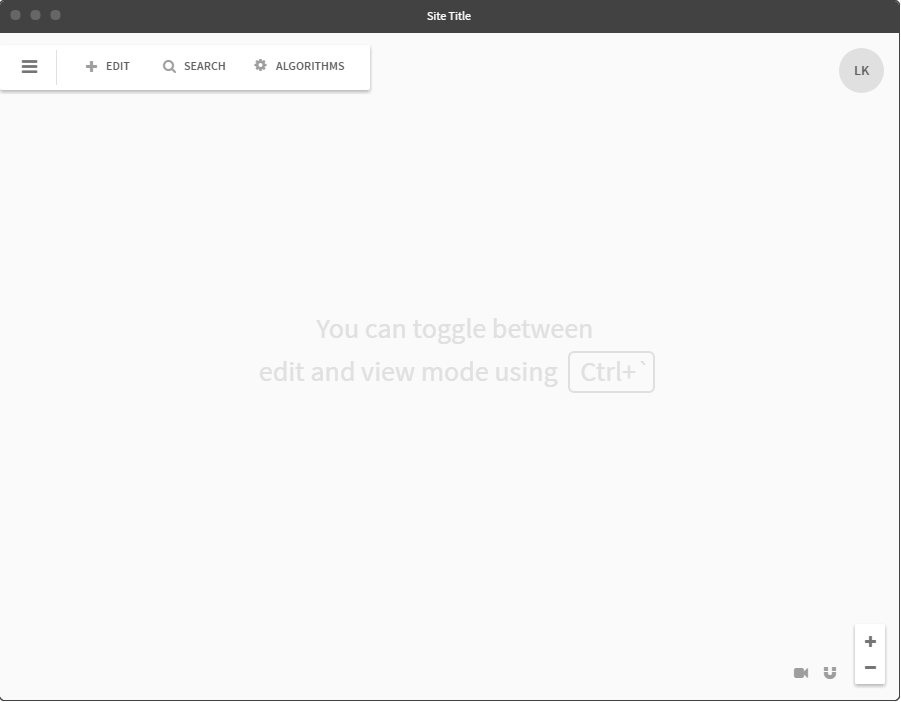
\includegraphics[width=\textwidth]{mock-view.png}
\caption{Tryb widoku grafu}
\end{figure}
\vspace*{\fill}

\pagebreak

\subsection*{Tryb edycji grafu}

Użytkownik powinien być poinformowany, że jest w trybie edycji poprzez oznaczenie przycisku oraz obramowania okna wyróżniającym się kolorem.

\vspace*{\fill}
\begin{figure}[H]
\centering
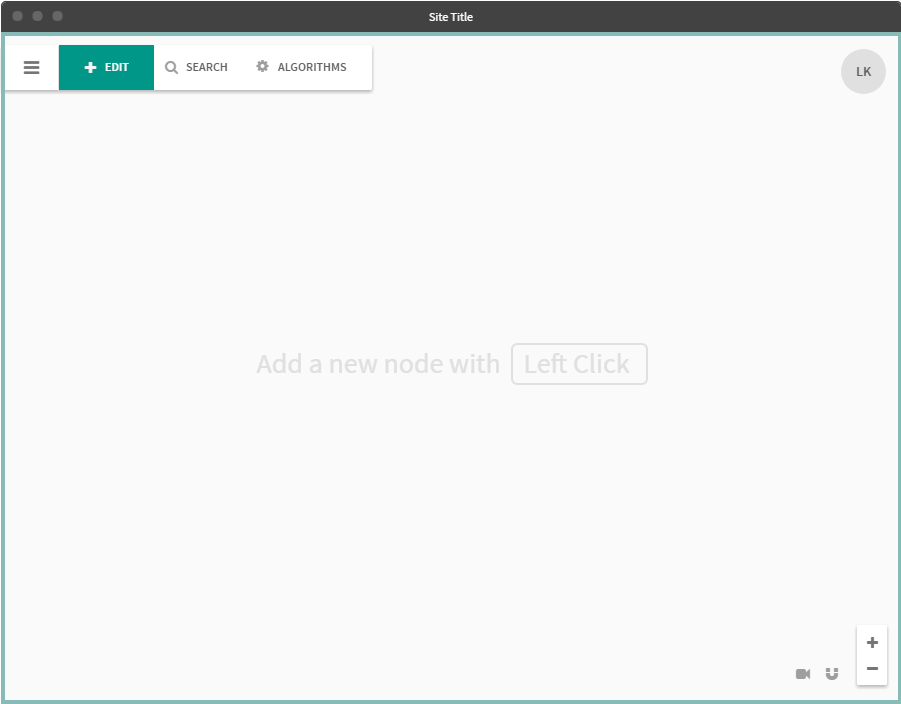
\includegraphics[width=\textwidth]{mock-edit.png}
\caption{Tryb edycji grafu}
\end{figure}
\vspace*{\fill}

\pagebreak

\subsection*{Widok menu}

Menu powinno wysuwać się z boku, a pod nim powinna pojawić się warstwa z półprzezroczystym tłem. Powinno oferować podstawowe opcje tworzenia nowego grafu, otwierania zapisanego grafu, udostępniania czy eksportowania. W menu powinny znaleźć się też takie opcje jak: wyświetlenie listy skrótów, zmiana języka, kontakt czy możliwość zgłoszenia błędu w aplikacji oraz informacja o prawach autorskich.

\vspace*{\fill}
\begin{figure}[H]
\centering
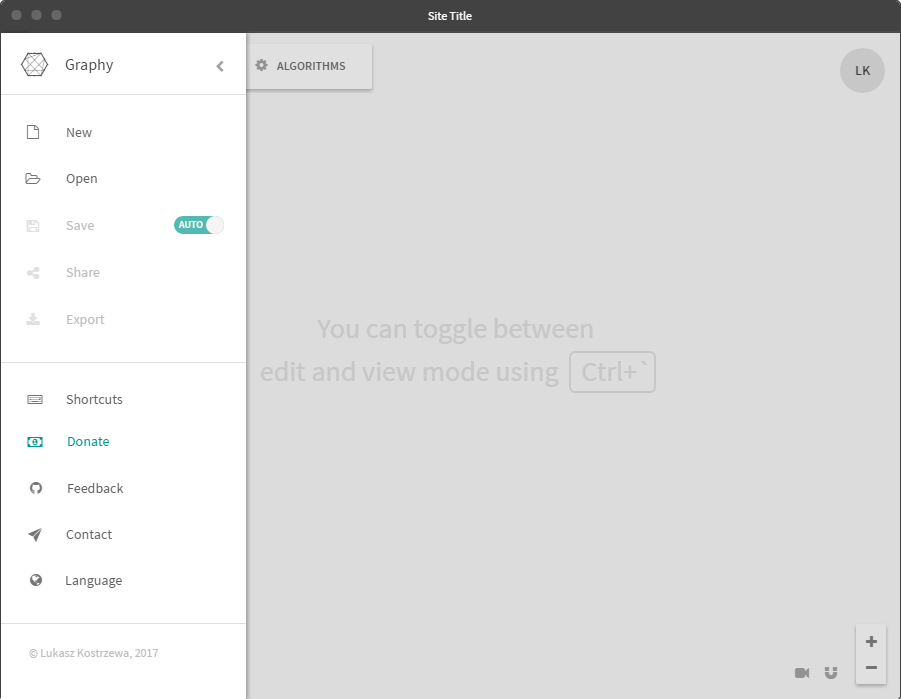
\includegraphics[width=\textwidth]{mock-menu.png}
\caption{Widok menu}
\end{figure}
\vspace*{\fill}

\pagebreak

\subsection*{Menu kontekstowe i informacja o ostatniej akcji}

Po kliknięciu prawego klawisza myszy powinno pojawić się niestandardowe menu kontekstowe zawierające dodatkowe opcje pozwalające na edycję, usuwanie, zaznaczanie, grupowanie, wycinanie, kopiowanie, wklejanie wierzchołków i krawędzi oraz na cofanie i ponawianie ostatniej akcji.

Po wykonaniu akcji modyfikującej graf na dole strony powinno wyświetlić się powiadomienie o wykonaniu tej akcji z przyciskiem umożliwiającym jej cofnięcie. 

\vspace*{\fill}
\begin{figure}[H]
\centering
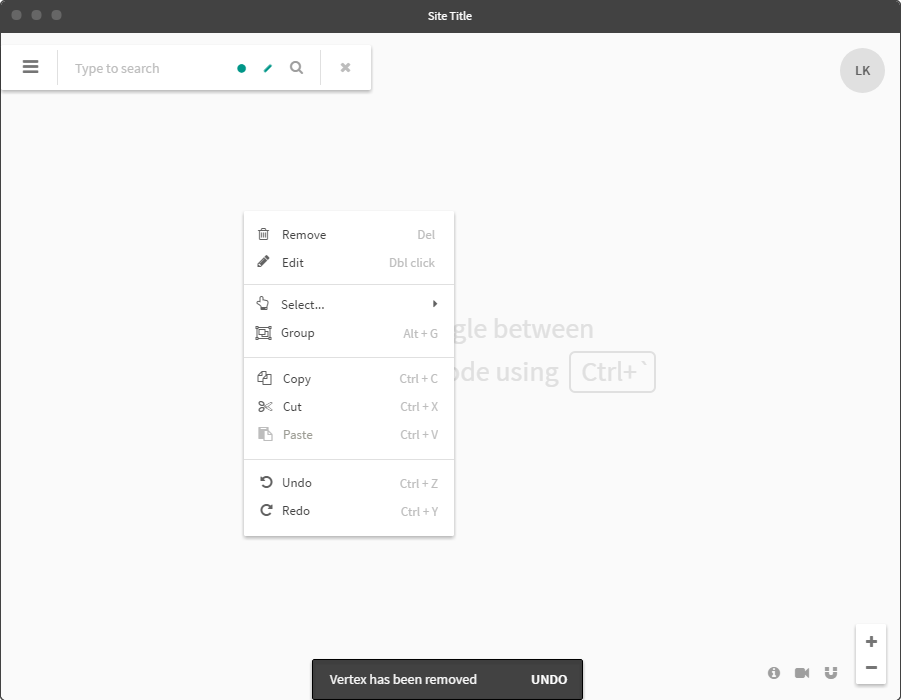
\includegraphics[width=\textwidth]{mock-context-menu.png}
\caption{Menu kontekstowe i informacja o ostatniej akcji}
\end{figure}
\vspace*{\fill}